%%%%%%%%%%%%%%%%%%%%%%%%%%%%%%%%%%%%%%%%%
% Classicthesis Typographic Thesis
% LaTeX Template
% Version 1.4 (1/1/16)
%
% This template has been downloaded from:
% http://www.LaTeXTemplates.com
%
% Original author:
% André Miede (http://www.miede.de) with commenting modifications by:
% Vel (vel@LaTeXTemplates.com)
%
% License:
% GNU General Public License (v2)
%
% General Tips:
% 1) Make sure to edit the classicthesis-config.file
% 2) New enumeration (A., B., C., etc in small caps): \begin{aenumerate} \end{aenumerate}
% 3) For margin notes: \marginpar or \graffito{}
% 4) Do not use bold fonts in this style, it is designed around them
% 5) Use tables as in the examples
% 6) See classicthesis-preamble.sty for useful commands
%
%%%%%%%%%%%%%%%%%%%%%%%%%%%%%%%%%%%%%%%%%

%----------------------------------------------------------------------------------------
%	PACKAGES AND OTHER DOCUMENT CONFIGURATIONS
%----------------------------------------------------------------------------------------

\documentclass[pdf]{beamer}
\usepackage[utf8]{inputenc}  % Em LaTeX clássico
\usepackage{listings}
\usepackage{lmodern}
\mode<presentation> {
  \usetheme{Madrid}
  %\usecolortheme{beaver}
}
\usepackage{amsmath}
\usepackage{listings}
\usepackage{minted}
\usepackage{caption}
\usepackage{tabularx} % Better tables
%\usepackage{enumitem}
\usepackage{multirow}
\usepackage{tikz}
\usetikzlibrary{arrows.meta}
\usetikzlibrary{positioning}
\usetikzlibrary{calc}
\usepackage{booktabs}
\usepackage{subcaption}

\tikzstyle{support}=[->,>=Latex,line width=1.5pt,color=blue!70]
\tikzstyle{defeat}=[->,>=Latex,line width=1.5pt,color=red!70]

% Beamer classic round bullets
\setbeamertemplate{items}[ball]
\setbeamertemplate{itemize items}[ball]

% Includes the file which contains all the document configurations and packages - make sure to edit this file
%\input{classicthesis-config}

%\addbibresource{Bibliography.bib} % The file housing your bibliography
%\addbibresource[label=ownpubs]{Self_Publications.bib} % Uncomment for optional self-publications

\title[TCC - 2/12/2025]{Probabilistic answer set programming for argumentation mining} % The short title appears at the bottom of every slide, the full title is only on the title page
\author{Jonas Rodrigues} % Your name
\institute[IME-USP] % Your institution as it will appear on the bottom of every slide, may be shorthand to save space
{
Universidade de São Paulo \\ % Your institution for the title page
\medskip
\textit{jonasrlg@ime.usp.br} \\ % Your email address
\medskip
Advisor: Prof.\ Denis Deratani Mauá\\
}
\date{\today} % Date, can be changed to a custom date

\begin{document}

\begin{frame}
\titlepage % Print the title page as the first slide
\end{frame}

\begin{frame}
\frametitle{Contents} % Table of contents slide, comment this block out to remove it
\tableofcontents % Throughout your presentation, if you choose to use \section{} and \subsection{} commands, these will automatically be printed on this slide as an overview of your presentation
\end{frame}

\section{Introduction}

\begin{frame}
    \frametitle{Probabilistic Logic Programming}
    \begin{minipage}[c]{0.5\linewidth}
        \begin{figure}
            \begin{center}
                \includegraphics[width=1.175\textwidth]{../thesis/gfx/problog.png}
            \end{center}
            \caption{Example of a ProbLog program, from Fierent et al. (2015).}
            \label{fig:problog}
        \end{figure}
    \end{minipage}
    \hfill
    \begin{minipage}[c]{0.4\linewidth}
        \centering
        % ------- Block: Probability of a total choice -------
        \begin{block}{Probability of a total choice}
            {\small
            A \textbf{total choice} $\Theta$ selects a subset of probabilistic facts.\\[2mm]
            }
            \[
            P(\Theta) =
            \prod_{f \in \Theta} p_f
            \prod_{f \notin \Theta}(1 - p_f)
            \]
        \end{block}

        % ------- Block: Probability of a query -------
        \begin{block}{Probability of a query}
            \[
            P(Q) = \sum_{\Theta : M_\Theta \models Q} P(\Theta)
            \]
            {\small
            Sum of all choices whose model makes $Q$ true.
            }
        \end{block}
    \end{minipage}
\end{frame}

\begin{frame}[fragile]{Knowledge Compilation}
        \begin{minted}{prolog}
    0.2::earthquake. 0.1::burglary. 0.5::hears(mary).
    alarm :- earthquake. alarm :- burglary.
    calls(mary) :- alarm, hears(mary).
        \end{minted}
        \vfill
        \centering
        \includegraphics[width=0.85\textwidth]{../thesis/gfx/slides/sdd2.pdf}
\end{frame}

% \subsection{Clark's Completion - Program to CNF}
% \begin{frame}[fragile]
%     \frametitle{Clark's Completion}
%     \begin{minipage}[c]{0.45\linewidth}
%     \centering
%     \begin{center}
%         \begin{minted}[fontsize=\Large]{prolog}
% 0.5::a.
% 0.5::b.
% c :- a, not b.
% c :- not a, b.
%         \end{minted}
%     \end{center}
%     \centering
%     \[
%     \bigwedge_{a \in \text{head}(P)}
%     \left(
%     a \iff
%     \bigvee_{\substack{B \in \text{body}(P) \\ a \leftarrow B \in P}}
%     \bigwedge_{b \in B} b
%     \right)
%     \]
%     \end{minipage}
%     \hfill
%     \begin{minipage}[c]{0.45\linewidth}
% \begin{minted}{text}
% p wcnf 5 9
% w 1 0.500000000 0
% w -1 0.500000000 0
% w 2 0.500000000 0
% w -2 0.500000000 0
% -4 3 0
% -4 1 0
% -4 -2 0
% 4 -1 2 0
% -5 3 0
% -5 2 0
% -5 -1 0
% 5 -2 1 0
% -3 4 5 0
% \end{minted}
%     \end{minipage}
% \end{frame}

\section{Preliminaries}

\subsection{Probabilistic Answer Set Programming}
\begin{frame}[fragile]
    \frametitle{Probabilistic Answer Set Programming (PASP)}
    \begin{minipage}[c]{0.45\linewidth}
        \begin{minted}{prolog}
0.5::b(1).
0.5::a(1).
x(1) :- a(1).
y(1,0); y(1,1) :- x(1).
y(1,0) :- b(1), not x(1).
y(1,1) :- not b(1), not x(1).
        \end{minted}
        \captionof{listing}{\textit{Non-stratified} PASP program,
        representing an Imprecise Hidden Markov Model.}
        \label{code:hmm}
    \end{minipage}
    \hfill
    \begin{minipage}[c]{0.45\linewidth}
        % Draw the equivalent HMM
        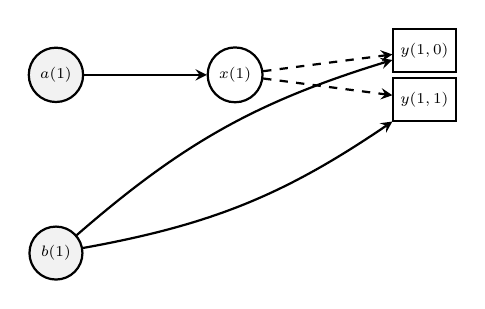
\begin{tikzpicture}[
          ->, >=stealth, thick,
          node distance=1.6cm,
          scale=0.78, transform shape,
          every node/.style={font=\scriptsize}
        ]

          % styles
          \tikzstyle{pfact}=[circle, draw, minimum size=6mm, fill=gray!10, align=center]
          \tikzstyle{state}=[circle, draw, minimum size=7mm, align=center]
          \tikzstyle{obs}=[rectangle, draw, minimum size=7mm, align=center]
          \tikzstyle{imp}=[->, dashed, thick]

          % probabilistic facts
          \node[pfact] (a1) {$a(1)$};
          \node[pfact, below=2cm of a1] (b1) {$b(1)$};

          % state literal
          \node[state, right=2.0cm of a1] (x1) {$x(1)$};

          % emitted literals
          \node[obs, right=2.1cm of x1, yshift=4mm] (y10) {$y(1,0)$};
          \node[obs, right=2.1cm of x1, yshift=-4mm] (y11) {$y(1,1)$};

          % edges
          \draw (a1) -- (x1);          % x(1) :- a(1).
          \draw[imp] (x1) -- (y10);    % choice when x(1)
          \draw[imp] (x1) -- (y11);

          \draw (b1) to[bend left=12] (y10);  % b(1), not x(1) -> y(1,0)
          \draw (b1) to[bend right=12] (y11); % not b(1), not x(1) -> y(1,1)

        \end{tikzpicture}
        \captionof{figure}{Graphical representation of the PASP Imprecise HMM program in Listing \ref{code:hmm}.}
    \end{minipage}
\end{frame}

% \begin{frame}
%     \frametitle{PASP Semantics}
%     \begin{block}{Max-Ent Semantics}
%     $$\mathbb{P}(\mathcal{M}) = \sum_{\theta : \mathcal{M} \in
%     \Gamma(\theta)} \frac{\mathbb{P}(\theta)}{\#StableModels(\theta)}$$
%     \end{block}
%     \vfill
%     \begin{block}{Credal Semantics (Upper and Lower)}
%     $$\overline{\mathbb{P}}(\mathcal{M}) = \sum_{\theta \in \Theta
%     : \Gamma(\theta) \cap \mathcal{M} \ne \emptyset} \mathbb{P}
%     (\theta), \qquad \underline{\mathbb{P}}(\mathcal{M}) = \sum_{\theta \in
%     \Theta : \Gamma(\theta) \subseteq \mathcal{M}} \mathbb{P}
%     (\theta)$$
%     \end{block}
% \end{frame}

\subsection{Negation Normal Form (NNF)}
\begin{frame}
    \frametitle{Negation Normal Form (NNF)}
    \begin{figure}[ht]
        \begin{minipage}[b]{0.45\linewidth}
            \centering
            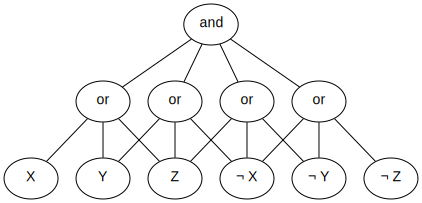
\includegraphics[width=1.1\textwidth]{../thesis/gfx/cnf.pdf}
            \caption{Example of a CNF formula in the NNF
            language.}
            \label{fig:cnf}
        \end{minipage}
        \hspace{0.5cm}
        \begin{minipage}[b]{0.45\linewidth}
            \centering
            \includegraphics[width=1.1\textwidth]{../thesis/gfx/dnf.pdf}
            \caption{Example of a DNF formula in the NNF
            language.}
            \label{fig:dnf}
        \end{minipage}
    \end{figure}
\end{frame}

\begin{frame}{GPU Parallelization}
    \centering
    \includegraphics[width=0.7\textwidth]{../thesis/gfx/slides/klay.png}
\end{frame}

% \begin{frame}
%     \frametitle{Structured (Decomposable) NNF}
%     \begin{figure}[ht]
%         \begin{minipage}[b]{0.45\linewidth}
%             \centering
%             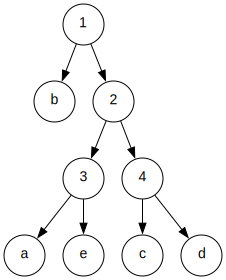
\includegraphics[width=\textwidth]{../thesis/gfx/vtree.pdf}
%             \caption{Example of a Vtree.}
%             \label{fig:vtree}
%         \end{minipage}
%         \hspace{0.5cm}
%         \begin{minipage}[b]{0.45\linewidth}
%             \centering
%             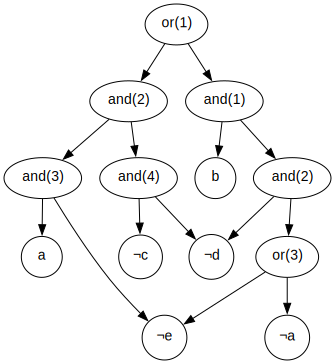
\includegraphics[width=\textwidth]{../thesis/gfx/dnnf_t_vtree.pdf}
%             \caption{A \textit{structured} DNNF formula for
%             $(\neg a \lor \neg e) \land (a \lor b) \land (b \lor
%             \neg c) \land (c \lor \neg d) \lor (\neg b \land
%             \neg d)$ that respects the Vtree in Figure
%             \ref{fig:vtree}.}
%             \label{fig:ddnf_t}
%         \end{minipage}
%     \end{figure}
% \end{frame}

% \begin{frame}
%     \frametitle{Sentential Decision Diagrams (SDDs)}
%     \begin{figure}[ht]
%         \begin{minipage}[b]{0.2\linewidth}
%             \centering
%             \includegraphics[width=\textwidth]{../thesis/gfx/sdd_apply1.pdf}
%             \caption{SDD representing $A \land B$.}
%             \label{fig:sdd_apply1}
%         \end{minipage}
%         \hspace{0.25cm}
%         \begin{minipage}[b]{0.25\linewidth}
%             \centering
%             \includegraphics[width=\textwidth]{../thesis/gfx/sdd_apply2.pdf}
%             \caption{SDD representing $\neg A \lor \neg C$.}
%             \label{fig:sdd_apply2}
%         \end{minipage}
%         \hspace{0.25cm}
%         \begin{minipage}[b]{0.45\linewidth}
%             \centering
%             \includegraphics[height=\textwidth]{../thesis/gfx/sdd_apply.pdf}
%             \caption{The result of the \textit{conjoin}
%             operation between the two SDDs.}
%             \label{fig:sdd_apply}
%         \end{minipage}
%     \end{figure}
% \end{frame}

% \begin{frame}[fragile]
%     \frametitle{Top-Down vs Bottom-Up KC}

%     \begin{minipage}[t]{0.45\linewidth}
%         \textbf{Top-Down}

%         \begin{minted}{text}
%     p cnf 5 9
%     -4 3 0
%     -4 1 0
%     -4 -2 0
%     4 -1 2 0
%     -5 3 0
%     -5 2 0
%     -5 -1 0
%     5 -2 1 0
%     -3 4 5 0
%         \end{minted}

%         \vspace{0.2cm}

%         \begin{itemize}
%             \item sd-DNNF (more succinct)
%             \item Introduces auxiliary variables
%             \item Fixed variable ordering
%         \end{itemize}
%     \end{minipage}
%     \hfill
%     \vrule width 0.5pt
%     \hfill
%     \begin{minipage}[t]{0.45\linewidth}
%         \textbf{Bottom-Up}

%         % Clark completion for this program
%         \[
%         \begin{aligned}
%         c &\iff (a \land \neg b) \lor  (\neg a \land b)
%         \end{aligned}
%         \]

%         \vspace{0.2cm}

%         \begin{itemize}
%             \item Uses SDDs (less succinct)
%             \item \textit{Apply} operator - no auxiliary variables needed
%             \item Dynamically optimized V-tree
%             \item Non-incremental compilation
%             \item Possibility of post-compilation re-ordering
%         \end{itemize}
%     \end{minipage}
% \end{frame}

\subsection{Argumentation}
\begin{frame}{Bipolar Argumentation Frameworks (BAF)}
    \centering

    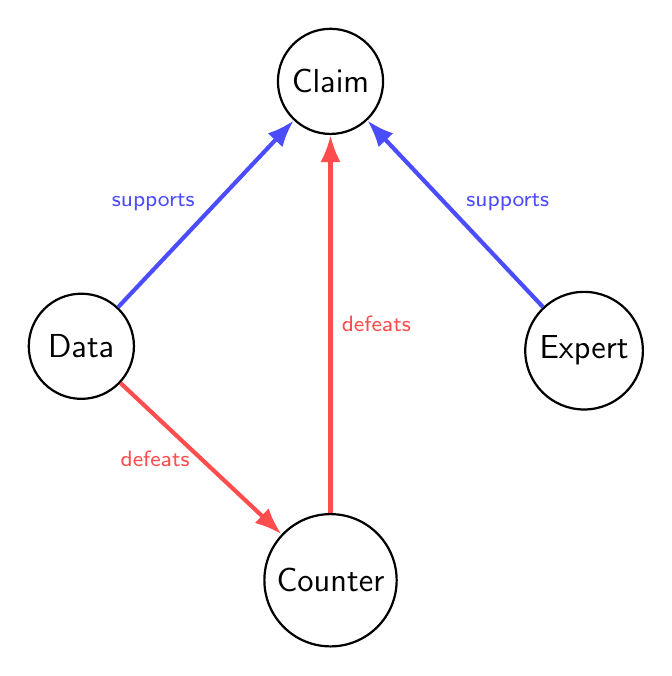
\begin{tikzpicture}[node distance=3.0cm]
    % tornar todos os nós do mesmo tamanho
    \tikzstyle{arg}=[draw,circle,thick,minimum size=38pt,font=\large\sffamily,fill=white]

    % espaçar mais os nós
    \node[arg] (claim) {Claim};
    \node[arg] (study) [below left=2.4cm and 2.2cm of claim] {Data};
    \node[arg] (expert) [below right=2.4cm and 2.2cm of claim] {Expert};
    \node[arg] (counter) [below=4.8cm of claim] {Counter};


    \draw[support] (study) -- node[left, font=\footnotesize\sffamily, yshift=4pt] {supports} (claim);
    \draw[support] (expert) -- node[right, font=\footnotesize\sffamily, yshift=4pt] {supports} (claim);
    \draw[defeat] (counter) -- node[right, font=\footnotesize\sffamily] {defeats} (claim);
    \draw[defeat] (study) -- node[left, font=\footnotesize\sffamily] {defeats} (counter);
    \end{tikzpicture}
\end{frame}

\section{Argumentation Compilation}
\begin{frame}{Proposal}
    \frametitle{Work Proposal}
    \begin{itemize}
        \item Pose the problem of inference in PASP with Argumentation as a
        second-level Algebraic Model Counting (2AMC):
        \begin{itemize}
            \item Compile a class of argumentation frameworks to Logic Circuits;
            \item Convert the sd-DNNF circuitos into Arithmetic Circuits for
            efficient inference.
        \end{itemize}
        \item Integrate the resulting circuit with auto-differentiation tools
        for end-to-end learning.
    \end{itemize}
    \centering
    \includegraphics[width=\textwidth]{../thesis/gfx/slides/diagram.pdf}
\end{frame}


% \subsection{Bottom-Up Compilation}
% \begin{frame}[fragile]
%     \frametitle{Bottom-Up Compilation}
%     \begin{minted}{prolog}
%         turing :- gödel, church.
%     \end{minted}
%     \begin{figure}
%         \begin{center}
%             \includegraphics[height=5cm]{../thesis/gfx/head_rule.pdf}
%         \end{center}
%         \caption{Compilation of the program above to an SDD with
%         balanced V-tree (with variable order as they appear in
%         the program).}
%         \label{fig:head_rule}
%     \end{figure}
% \end{frame}

% \begin{frame}[fragile]
%     \frametitle{Bottom-Up Compilation}
%     \begin{minted}{prolog}
%         knuth :- pólya, church.
%         knuth :- vonNeumann.
%     \end{minted}
%     \begin{figure}[ht]
%         \begin{minipage}[b]{0.45\linewidth}
%             \centering
%             \includegraphics[width=0.64\textwidth]{../thesis/gfx/multiple_head_body.pdf}
%             \caption{SDD representing $polya \land church$.}
%             \label{fig:multiple_head_body}
%         \end{minipage}
%         \hspace{0.5cm}
%         \begin{minipage}[b]{0.45\linewidth}
%             \centering
%             \includegraphics[width=\textwidth]{../thesis/gfx/multiple_head.pdf}
%             \caption{The result of the \textit{iff} operation
%             between $knuth \iff (polya \land church) \lor
%             vonNeumann$.}
%             \label{fig:multiple_head}
%         \end{minipage}
%     \end{figure}
% \end{frame}

% \begin{frame}[fragile]
%     \frametitle{Bottom-Up Compilation}
%     \centering
%     \begin{center}
%         \begin{minted}{prolog}
%             turing :- gödel, church.
%             knuth :- polya, church.
%             knuth :- vonNeumann.
%         \end{minted}
%     \end{center}
%     \begin{figure}
%         \begin{center}
%             \includegraphics[height=5cm]{../thesis/gfx/rule_by_rule.pdf}
%         \end{center}
%         \caption{Conjoin of the circuits in Figures
%         \ref{fig:head_rule} and \ref{fig:multiple_head}.}
%     \end{figure}
% \end{frame}

% \begin{frame}
%     \frametitle{smProbLog Compilation - Top Down}
%     \begin{figure}
%         \begin{center}
%             \includegraphics[width=0.6\textwidth]{../thesis/gfx/smproblog_circuit.pdf}
%         \end{center}
%         \caption{PASP (or smProblog) compilation example, by
%         Pietro Totis, Angelika Kimmig, Luc De Raedt}
%         \label{fig:smproblog_circuit}
%     \end{figure}
% \end{frame}

% \begin{frame}
%     \frametitle{smProbLog Enumeration}
%     \begin{figure}
%         \begin{center}
%             \includegraphics[width=0.6\textwidth]{../thesis/gfx/smproblog_enum.pdf}
%         \end{center}
%         \caption{PASP (or smProblog) enumeration example, by
%         Pietro Totis, Angelika Kimmig, Luc De Raedt}
%         \label{fig:smproblog_enum}
%     \end{figure}
% \end{frame}

% \begin{frame}[fragile]
%     \frametitle{PASP Bottom-Up Compilation}
%     \begin{block}{Integrity Constraints}
%         \begin{minted}{prolog}
% :- b1, b2, ..., not c1, not c2, ...
%         \end{minted}
%         \vspace{-1em}
%         \rule{\linewidth}{0.4pt}
%         \vspace{-1em}
%         \[
%         \neg \left ( b_1 \land b_2 \land ... \land \neg c_1 \land \neg c_2 \land ...
%         \right ) = \neg b_1 \lor \neg b_2 \lor ... \lor c_1 \lor c_2 \lor ...
%         \]
%     \end{block}

%     \begin{block}{Disjunctive Rules}
%         \begin{minted}{prolog}
% a1; ...; an :- b1, b2, ..., not c1, not c2, ...
%         \end{minted}
%         \vspace{-1em}
%         \rule{\linewidth}{0.4pt}
%         \vspace{-1em}
%         \begin{minted}{prolog}
% a1 :- b1, b2, ..., not c1, not c2, ..., not a2, ... , not an.
% ...
% an :- b1, b2, ..., not c1, not c2, ..., not a1, ...
%         \end{minted}
%     \end{block}

%     \begin{block}{Cardinality Constraints}
%         \begin{minted}{prolog}
% {a1, a2, ..., an} u.
%         \end{minted}
%         \vspace{-1em}
%         \rule{\linewidth}{0.4pt}
%         \vspace{-1em}
%         \[
%         \text{Upper}(A, 0, u) = \textsc{ITE}(a1, \text{Upper}(A \setminus \{a1\}, 1, u), \text{Upper}(A \setminus \{a1\}, 0, u))
%         \]
%     \end{block}
% \end{frame}

% \begin{frame}
%     \frametitle{Tractable PASP Inference with Circuits}
%     \begin{block}{Algebraic Model Counting (AMC)}
%     $$A(T) = \bigoplus_{I \in \mathcal{M}(T)} \bigotimes_{i \in
%     I} \alpha(i)$$
%     Example: ProbLog inference (weighted model counting).
%     \end{block}
%     \begin{block}{Second-Level Algebraic Model Counting (2AMC)}
%     $$2AMC(T) = \bigoplus_{\mathbf{a} \in A(X_O)}^O
%                 \bigotimes_{a \in \mathbf{a}}^O \alpha_O(a)
%                 \otimes_O t
%                 \left (
%                 \bigoplus_{I \in \mathcal{M}(T|\mathbf{a})}^I
%                 \bigotimes_{i \in I}^I \alpha_I(i) \right )$$
%     Examples: Inference in PASP (Max-Ent and Credal semantics).
%     \end{block}
%     \begin{block}{Benjie Wang, Denis Mauá, Guy Van den Broeck, YooJung Choi}
%     $X$-determinism is both necessary and sufficient for tractable PASP
%     inference using Arithmetic Circuits.
%     \end{block}
% \end{frame}

% \subsection{V-Tree Optimization}
% \begin{frame}
%     \frametitle{Impact of Variable Ordering}
%     \begin{figure}[ht]
%         \begin{minipage}[b]{0.45\linewidth}
%             \centering
%             \includegraphics[width=0.75\textwidth]{../thesis/gfx/hmm_left.pdf}
%             \caption{Bottom-Up compilation of the Program
%             \ref{code:hmm} following a left-linear V-tree.}
%             \label{fig:hmm_left}
%         \end{minipage}
%         \hspace{0.5cm}
%         \begin{minipage}[b]{0.45\linewidth}
%             \centering
%             \includegraphics[width=0.85\textwidth]{../thesis/gfx/hmm_right.pdf}
%             \caption{Bottom-Up compilation of the Program
%             \ref{code:hmm} following a right-linear V-tree.}
%             \label{fig:hmm_right}
%         \end{minipage}
%     \end{figure}
% \end{frame}

% \begin{frame}[fragile]
%     \frametitle{V-Tree Optimization}

%     \centering
%     \begin{minipage}[c]{0.45\linewidth}
%         \centering
%         \begin{minted}[fontsize=\Large]{prolog}
%       0.5::a. 0.5::x.
%       b :- a. y :- x.
%       c :- b. z :- y.
%       j :- c, not z.
%         \end{minted}
%     \end{minipage}
%     \hfill
%     \begin{minipage}[c]{0.45\linewidth}
%         \centering
%         \begin{tikzpicture}[->,>=stealth, node distance=1.2cm]

%             % Styles
%             \tikzstyle{bluenode}=[circle, draw, fill=blue!50, minimum size=7mm]
%             \tikzstyle{softbluenode}=[circle, draw, fill=blue!30, minimum size=7mm]
%             \tikzstyle{lighterbluenode}=[circle, draw, fill=blue!10, minimum size=7mm]
%             \tikzstyle{plainnode}=[circle, draw, fill=white, minimum size=7mm]

%             % Top level
%             \node[bluenode] (a) {a};
%             \node[bluenode, right=1.5cm of a] (x) {x};

%             % Middle level
%             \node[softbluenode, below=1.2cm of a] (b) {b};
%             \node[softbluenode, below=1.2cm of x] (y) {y};

%             % Second last level
%             \node[lighterbluenode, below=1.2cm of b] (c) {c};
%             \node[lighterbluenode, below=1.2cm of y] (z) {z};

%             % Final level
%             \node[plainnode, below=1.2cm of c, xshift=1.2cm] (j) {j};

%             % Edges
%             \draw (a) -- (b);
%             \draw (b) -- (c);
%             \draw (x) -- (y);
%             \draw (y) -- (z);
%             \draw (c) -- (j);
%             \draw (z) -- (j);

%         \end{tikzpicture}
%     \end{minipage}
% \end{frame}

% \begin{frame}
%     \frametitle{Variables Initialization - Experimental Results}
%     \begin{table}
%         \centering
%         \begin{tabular}{crrrrrr}
%             \toprule
%             \multirow{2}{*}{\#Nodes} & \multicolumn{2}{c}{Proposed} & \multicolumn{2}{c}{MinDegree} & \multicolumn{2}{c}{MinFill} \\
%             & mb & s & mb & s & mb & s \\
%             \midrule
%             %12 & \textbf{272} & \textbf{0.72} & 1608 & 6.91 & 385 & 1.17 \\
%             13 & \textbf{374} & \textbf{2.42} & 10020 & 229 & 805 & 4.07 \\
%             14 & \textbf{387} & \textbf{5.48} & - & - & 754 & 7.21 \\
%             15 & \textbf{997} & 32.2 & - & - & 2939 & \textbf{31.99} \\
%             16 & \textbf{9640} & \textbf{279} & - & - & - & - \\
%             17 & \textbf{10411} & \textbf{588} & - & - & - & - \\
%             \bottomrule
%         \end{tabular}%
%         \caption{Comparison of memory (\textbf{mb}) and time (\textbf{s}econds) between the proposed
%         heuristic, MinDegree and MinFill for $V$-tree initialization, in the \textbf{Coloring} dataset
%         for bottom-up compilation.}
%         \label{tab:vtree-comparison}
%     \end{table}
% \end{frame}

% \begin{frame}{Dynamic Minimization}
%     \centering
%     \includegraphics[width=0.7\textwidth]{../thesis/gfx/slides/Swap.png}
% \end{frame}

% \subsection{Non-Incremental Compilation}

% \begin{frame}[fragile]
%     \frametitle{Non-Incremental Compilation}

%     \begin{minipage}[c]{0.45\linewidth}
%         \centering
%         \begin{minted}[fontsize=\Large]{prolog}
%       0.5::a. 0.5::x.
%       b :- a. y :- x.
%       c :- b. z :- y.
%       j :- c, not z.
%         \end{minted}
%     \end{minipage}
%     \hspace{0.5cm}
%     \begin{minipage}[c]{0.45\linewidth}
%         \centering
%         \begin{tikzpicture}[->,>=stealth, node distance=1.2cm]

%             % Styles
%             \tikzstyle{bluenode}=[circle, draw, fill=blue!20, minimum size=7mm]
%             \tikzstyle{rednode}=[circle, draw, fill=red!20, minimum size=7mm]
%             \tikzstyle{plainnode}=[circle, draw, minimum size=7mm]

%             % Top level
%             \node[bluenode] (a) {a};
%             \node[rednode, right=1.5cm of a] (x) {x};

%             % Middle level
%             \node[bluenode, below=1.2cm of a] (b) {b};
%             \node[rednode, below=1.2cm of x] (y) {y};

%             % Second last level
%             \node[bluenode, below=1.2cm of b] (c) {c};
%             \node[rednode, below=1.2cm of y] (z) {z};

%             % Final level
%             \node[plainnode, below=1.2cm of c, xshift=1.2cm] (j) {j};

%             % Edges
%             \draw (a) -- (b);
%             \draw (b) -- (c);
%             \draw (x) -- (y);
%             \draw (y) -- (z);
%             \draw (c) -- (j);
%             \draw (z) -- (j);

%         \end{tikzpicture}
%     \end{minipage}
% \end{frame}

% \begin{frame}{Non-Incremental KC - Experimental Results}
%     \begin{figure}
%         \centering
%         \begin{subfigure}{0.48\linewidth}
%             \centering
%             \includegraphics[width=\linewidth]{../thesis/gfx/non_inc/coloring_time_non_inc.pdf}
%             \caption{Compilation time (seconds).}
%             \label{fig:non_inc_time}
%         \end{subfigure}
%         \hfill
%         \begin{subfigure}{0.48\linewidth}
%             \centering
%             \includegraphics[width=\linewidth]{../thesis/gfx/non_inc/coloring_mb_non_inc.pdf}
%             \caption{Peak memory usage (mb).}
%             \label{fig:non_inc_mem}
%         \end{subfigure}

%         \caption{Comparison between incremental (y-axis) and non-incremental (x-axis)
%         compilation as we increase the number of nodes (darker colors) of the graph
%         \textsc{Coloring} program.}
%         \label{fig:non_inc}
%     \end{figure}
% \end{frame}

% \subsection{Experimental Results}

% \begin{frame}
%   \frametitle{Non-Incremental vs Top-Down KC}
%   \begin{figure}
%       \begin{subfigure}{0.48\linewidth}
%         \centering
%         \includegraphics[width=0.7\linewidth]{../thesis/gfx/best/Vtree_irl.pdf}
%         \caption{IRL}
%         \label{fig:best_irl}
%       \end{subfigure}
%       \hfill
%       \begin{subfigure}{0.48\linewidth}
%         \centering
%         \includegraphics[width=0.7\linewidth]{../thesis/gfx/best/Vtree_irn.pdf}
%         \caption{IRN}
%         \label{fig:best_irn}
%       \end{subfigure}
%       \vspace{0.5em}
%       \begin{subfigure}{0.48\linewidth}
%         \centering
%         \includegraphics[width=0.7\linewidth]{../thesis/gfx/best/Vtree_coloring.pdf}
%         \caption{Coloring}
%         \label{fig:best_coloring}
%       \end{subfigure}
%       \hfill
%       \begin{subfigure}{0.48\linewidth}
%         \centering
%         \includegraphics[width=0.7\linewidth]{../thesis/gfx/best/Vtree_pin_complete_best.pdf}
%         \caption{PIN Complete}
%         \label{fig:best_pin_complete}
%       \end{subfigure}
%       % \caption{Comparison of circuit size for the Non-Incremental bottom-up
%       % compilation across eight different datasets. The x-axis and y-axis represent,
%       % respectively, the size of the circuit produced by a compiler and the instance size. Cyan
%       % and magenta represent, respectively, constrained and Non-Incremental compilation with dynamic
%       % re-ordering. Datasets where the cyan dots are consistently over the magenta represent scenarios
%       % imposing $X$-constrainedness had a heavy impact on circuit size.}
%       % \label{fig:best}
%       \caption{Comparison of circuit size between bottom-up (black) and top-down compilers:
%       \textsc{c2d} (cyan), \textsc{d4} (magenta), \textsc{SharpSAT-TD} (yellow).}
%     \end{figure}
% \end{frame}

% \section{Future Work}
% \begin{frame}{Opportunities - Dual Compilation}
%     \centering
%     \begin{figure}
%         \centering
%         \includegraphics[width=0.7\textwidth]{../thesis/gfx/unconstrained/Vtree_pin_best.pdf}
%         \caption{Comparison of circuit size for the unconstrained (cyan) and $X$-constrained (magenta)
%         bottom-up compilation for the Smokers dataset.}
%         \label{fig:unconstrained_vs_constrained}
%     \end{figure}
% \end{frame}

\begin{frame}
\Huge{\centerline{The End}}
\Huge{\centerline{Thank You!}}
\end{frame}

\end{document}
